\documentclass[hyperref={pdfpagelabels=false},xcolor={dvipsnames},compress,table,usenames,dvipsnames]{beamer}
\usepackage{lmodern}
\usepackage{svg}
\usepackage{listings}

\lstdefinelanguage{swift}
{
  morekeywords={
    open,catch,@escaping,nil,throws,func,if,then,else,for,in,while,do,switch,case,default,where,break,continue,fallthrough,return,
    typealias,struct,class,enum,protocol,var,func,let,get,set,willSet,didSet,inout,init,deinit,extension,
    subscript,prefix,operator,infix,postfix,precedence,associativity,left,right,none,convenience,dynamic,
    final,lazy,mutating,nonmutating,optional,override,required,static,unowned,safe,weak,internal,
    private,public,is,as,self,unsafe,dynamicType,true,false,nil,Type,Protocol,
  },
  morecomment=[l]{//}, % l is for line comment
  morecomment=[s]{/*}{*/}, % s is for start and end delimiter
  morestring=[b]", % defines that strings are enclosed in double quotes
  breaklines=true,
  escapeinside={\%*}{*)},
  numbers=none,
  captionpos=b,
  breakatwhitespace=true,
  basicstyle=\linespread{1.0}\ttfamily\footnotesize, % https://tex.stackexchange.com/a/102728/129441
}

\definecolor{keyword}{HTML}{BA2CA3}
\definecolor{string}{HTML}{D12F1B}
\definecolor{comment}{HTML}{008400}

\lstset{
  language=swift,
  inputencoding=utf8,
  extendedchars=\true,
  basicstyle=\ttfamily\small,
  showstringspaces=false, % lets spaces in strings appear as real spaces
  columns=fixed,
  keepspaces=true,
  keywordstyle=\color{keyword},
  stringstyle=\color{string},
  commentstyle=\color{comment}
}

\usetheme{Berlin}

\AtBeginSection[]{
    \begin{frame}
        \vfill
        \centering
        \begin{beamercolorbox}[sep=8pt,center,shadow=false,rounded=false]{title}
            \usebeamerfont{title}\insertsectionhead\par%
        \end{beamercolorbox}
        \vfill
    \end{frame}
}

\title{The art of inlining}
\author{Maciej Procyk}
\date{May 9, 2022}
\begin{document}

    \logo{
\includegraphics[width=180pt]{images/logo.png}}

    {
        \setbeamertemplate{logo}{}
        \setbeamertemplate{headline}{}
        \begin{frame}
            \maketitle
        \end{frame}
    }


    \begin{frame}
        \frametitle{Table of contents}
        \tableofcontents
    \end{frame}


    \section{Introduction}

    \subsection{Practical usage}

    \begin{frame}[fragile]{The goal of the story}
        \begin{center}
            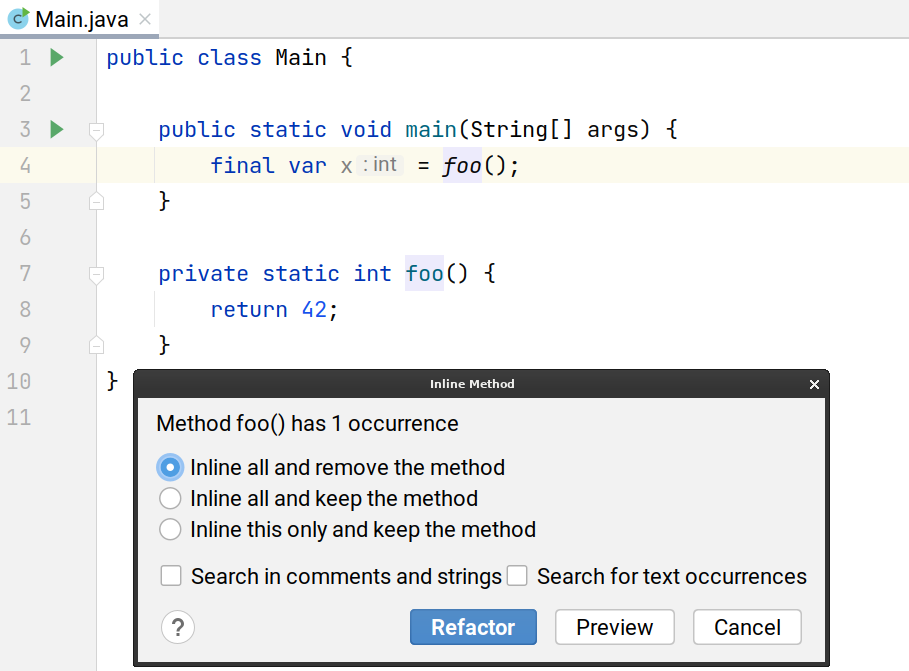
\includegraphics[width=180pt]{images/goal.png}
        \end{center}
        \uncover<2->{Adding similar (or better) support for Swift language seems to be pretty easy}
        \uncover<3->{but the devil is in the (implementation) details.}
    \end{frame}

    \subsection{Problem background}

    \begin{frame}{Inline method refactoring dialog in Intellij}
        \begin{itemize}
            \uncover<1->{\item available only for most popular languages including Java and Kotlin}
            \uncover<2->{\item action placing method's body into the body of its callers}
            \uncover<3->{\item can inline the occurrences and remove/leave the method definition}
            \uncover<4->{\item searches for method references in comments, strings and documentation}
            \uncover<5->{\item handful in bigger refactoring with huge codebase}
        \end{itemize}
    \end{frame}

    \section{Inlining problem}

    \subsection{Back to the root of the problem}

    \begin{frame}{Researched problem of inlining in GHC}
        \begin{itemize}
            \uncover<1->{\item based on paper "Secrets of the Glasgow Haskell Compiler inliner" by Simon Peyton Jones and Simon Marlow}\uncover<2->{ published in 1999}
            \uncover<3->{\item learn from the lesson of other developers}
            \uncover<4->{\item get familiar with solutions and problems existing in "production" inliner}
            \uncover<5->{\item get familiar with the abstraction of inlining}   
        \end{itemize}
    \end{frame}

    \begin{frame}{Main interesting issues}
        \begin{itemize}
            \uncover<1->{\item name capturing - found simple alternative to the inconvenient process of plumbing}
            \uncover<2->{\item improving conservative approach to recursive definitions}
            \uncover<3->{\item taking into account the time cost of inlining (being aware of exponential cost)}
            \uncover<4->{\item inlining an expression $\Rightarrow$ retain the expression's lexical environment}\uncover<5->{ tracking of both lexical and dynamic environments}
        \end{itemize}
    \end{frame}


    \subsection{Process of inlining}

    \begin{frame}[fragile]{Basic example}
        \begin{exampleblock}
            <1->{basic-inline.hs}
            \begin{lstlisting}
let { f = \x -> x * 3 } in f (a + b) - c
==>
(a + b) * 3 - c
            \end{lstlisting}
        \end{exampleblock}
        where $\texttt{==>}$, following paper convention, indicates a program transformation
    \end{frame}


    \begin{frame}{Indentified transformations informally are described as "inlining"}
        \begin{enumerate}
            \uncover<1->{\item \textit{inlining itself} replaces an occurrence of a \texttt{let}-bound variable by (a copy of) the right-hand side of its definition}
            \uncover<2->{\item \textit{dead code elimination} discards bindings that are no longer used - occurs when all occurrences of a variable have been inlined}
            \uncover<3->{\item \textit{$\beta$-reduction} simply rewrites a lambda application \texttt{($\backslash$x->E) A} to \texttt{let \{x = A\} in E}}
        \end{enumerate}
    \end{frame}

    \begin{frame}[fragile]{Transformations}
        \begin{enumerate}
        \setcounter{enumi}{0}
        \item Inlining itself
        \end{enumerate}
        \begin{exampleblock}
            <1->{inlining-itself.hs}
            \begin{lstlisting}
let { f = \x -> x * 3 } in f (a + b) - c
==> [inline f]
let { f = \x -> x * 3 } in
  (\x -> x * 3) (a + b) - c
            \end{lstlisting}
        \end{exampleblock}
    \end{frame}
    
    \begin{frame}[fragile]{Transformations}
        \begin{enumerate}
        \setcounter{enumi}{1}
        \item Dead code elimination
        \end{enumerate}
        \begin{exampleblock}
            <1->{dead-code-elimination.hs}
            \begin{lstlisting}
let { f = \x -> x * 3 } in
  (\x -> x * 3) (a + b) - c
==> [dead f]
(\x -> x * 3) (a + b) - c
            \end{lstlisting}
        \end{exampleblock}
    \end{frame}
    
    \begin{frame}[fragile]{Transformations}
        \begin{enumerate}
        \setcounter{enumi}{2}
        \item $\beta$-reduction
        \end{enumerate}
        \begin{exampleblock}
            <1->{beta-reduction.hs}
            \begin{lstlisting}
(\x -> x * 3) (a + b) - c
==> [beta]
(let { x = a + b } in x * 3) - c
            \end{lstlisting}
        \end{exampleblock}
    \end{frame}

    \begin{frame}{Factors affecting inlining}
        \begin{itemize}
            \item Does any code get duplicated? If so, then how much? \pause
            \item GHC uses multiple heuristics to determine whether expression is small enough to be duplicated
        \end{itemize}
    \end{frame}

    \begin{frame}[fragile]{Factors affecting inlining}
        \begin{itemize}
            \item Does any work get duplicated?
        \end{itemize}
        \begin{exampleblock}
            <2->{obvious-duplicate.hs}
            \begin{lstlisting}
let x = foo 1000 in x + x
            \end{lstlisting}
        \end{exampleblock}
        \begin{exampleblock}
            <3->{careful-duplicate.hs}
            \begin{lstlisting}
let x = foo 1000
f = \y -> x * y
in ...(f 3)..(f 4)...
            \end{lstlisting}
        \end{exampleblock}
    \end{frame}

    \begin{frame}[fragile]{Factors affecting inlining}
        \begin{itemize}
            \item Are any transformations exposed by inlining?
        \end{itemize}
        \begin{exampleblock}
            <2->{exposed-transformation.hs}
            \begin{lstlisting}
f = \x -> E
g = \ys -> map f ys
==>
g = \ys -> map (\x -> E) ys
            \end{lstlisting}
        \end{exampleblock}
        \uncover<3->{the closure for \texttt{($\backslash$ x -> E)} would have to b e allocated each time \texttt{g} was called}
    \end{frame}

    \begin{frame}[fragile]{General conclusions about inlining}
        \begin{itemize}
            \item is not an optimization by itself\pause
            \item may duplicate code or work\pause
            \item saves a call jump (not always as on the last example)\pause
            \item exposes new transformations by bringing together two code fragments that were separate
        \end{itemize}
    \end{frame}

    \subsection{Name capturing}

    \begin{frame}[fragile]{Name capturing problems}
        \begin{exampleblock}
            <1->{wrong-naming.hs}
            \begin{lstlisting}
let x = a + b in
  let a = 7 in
    x + a
==>
let a = 7 in (a + b) + a
            \end{lstlisting}
        \end{exampleblock}
    \end{frame}

    \begin{frame}[fragile]{Dealing with name capturing - sledge hammer}
        \begin{itemize}
            \item rename all bound variables during inlining process\pause
            \item allocates much more fresh names than are actually necessary\pause
            \item slow downs the compilation process\pause
            \item painful getting name source to where it's needed\uncover<5->{ - situation only different in cosmetics when monads are used}
        \end{itemize}
    \end{frame}

    \begin{frame}[fragile]{Dealing with name capturing - the rappier}
        \begin{itemize}
            \item let \textit{subst M [E$\backslash$x]} mean substitution of \textit{E} for \textit{x} in \textit{M}\pause
            \item then \textit{subst ($\lambda$x. M) [E$\backslash$x] = $\lambda$x. M}\pause
            \item then \textit{subst ($\lambda$x. M) [E$\backslash$y] = $\lambda$x. (subst M [E$\backslash$y])\\if x doesn't occur free in E else rename x}\pause
            \item we need to know the free variables of \textit{E} (range of the substitution) - might be costly to compute\pause
            \item \textit{no-shadowing strategy} - renaming any bound variable for which there was an enclosing binding (all variables in scope)
        \end{itemize}
    \end{frame}

    \begin{frame}[fragile]{Dealing with name capturing - final rules}
        \begin{itemize}
            \item let $\theta$ be a set of in-scope variables and $\phi$ a substitution\pause
            \item \textit{subst ($\lambda$x. M) $\phi$ $\theta$ = $\lambda$x. (subst M $(\phi\backslash x)$ $(\theta \cup \lbrace x \rbrace)$) if $x\not\in \theta$}\pause
            \item \textit{subst ($\lambda$x. M) $\phi$ $\theta$ = $\lambda$y. (subst M $\phi[x \mapsto y]$ $(\theta \cup \lbrace y \rbrace)$) if $x\in \theta$ where $y\not\in \theta$}
        \end{itemize}
    \end{frame}

    \begin{frame}[fragile]{Dealing with name capturing - choosing name}
        \begin{itemize}
            \item trying \textit{x1, x2} and so on names there is a danger of repeating the search if a lot of names are in scope\pause
            \item we may compute a hash value of in-scope variables and use it to create a name\pause
            \item indeed, using the number of enclosing binders gives something not unlike de Bruijn numbers
        \end{itemize}
    \end{frame}

    \begin{frame}[fragile]{Choosing a name - other approaches}
        \begin{itemize}
            \item using de Bruijn numbers to name the variables\pause
            \item disadvantage - pushing a substitution inside a lambda, needs adjustment of entire range of the substitution (which should be done lazily)\pause
            \item introduces quite more administration in compiler code
        \end{itemize}
    \end{frame}

    \section{Swift flavors}

    \subsection{Swift introduction}

    \begin{frame}[fragile]{Swift language}
        \begin{itemize}
            \item programming language for iOS, macOS, watchOS, and tvOS app development\pause
            \item a type-safe language developed as a replacement for Objective-C\pause
            \item uses the Objective-C runtime library, which allows C, Objective-C, C++ and Swift code to run within one program\pause
            \item built with the LLVM compiler framework\pause
            \item protocol-oriented programming (similar to interfaces and traits)
        \end{itemize}
    \end{frame}

    \subsection{Planned implementation}

    \begin{frame}[fragile]{Main assumptions}
        \begin{itemize}
            \item inlining process done before compilation process\pause
            \item induced by user (software engineer) but may affect multiple places\pause
            \item may include suggestions when it's recommended to inline the function
        \end{itemize}
    \end{frame}

    \subsection{Found corner cases}

    \begin{frame}[fragile]{Name shadowing}
        \begin{exampleblock}
            <1->{name-shadowing.swift}
            \begin{lstlisting}
func f() -> Int {
    var x = 24
    return x + 42
}
func g() -> Int {
    var x = 42
    return x + 24
}
let x = f() + g()
            \end{lstlisting}
        \end{exampleblock}
    \end{frame}

    \begin{frame}[fragile]{Early returns}
        \begin{exampleblock}
            <1->{early-returns.swift}
            \begin{lstlisting}
func f(x: Int) -> Int {
    if x == 24 {
        return 0
    }
    return 42
}
let x = f(x: 24)
            \end{lstlisting}
        \end{exampleblock}
    \end{frame}

    \begin{frame}[fragile]{Explicit typing}
        \begin{exampleblock}
            <1->{explicit-typing.swift}
            \begin{lstlisting}
func f() -> Double { 0 }
let x = f()  
// is different than 
let y = 0
            \end{lstlisting}
        \end{exampleblock}
    \end{frame}

    \begin{frame}[fragile]{Nested functions inlining}
        \begin{exampleblock}
            <1->{nested-functions.swift}
            \begin{lstlisting}
func f(y: Int) -> Int {
    func g(x: Int) -> Int { 24 + x + y }
    return g(x: 42 + y)
}
let x = f(y: 24)
            \end{lstlisting}
        \end{exampleblock}
    \end{frame}

    \begin{frame}[fragile]{Generics and inout params}
        \begin{exampleblock}
            <1->{generics-inout.swift}
            \begin{lstlisting}
func swap<T>(_ a: inout T, _ b: inout T) {
    let aux = a
    a = b
    b = aux
}
var x = 42
var y = 24
swap(&x, &y)
            \end{lstlisting}
        \end{exampleblock}
    \end{frame}

    \begin{frame}[fragile]{Named params}
        \begin{exampleblock}
            <1->{named-params.swift}
            \begin{lstlisting}
func f(x: Int) -> Int { x }

func g(_ x: Int) -> Int { x }

func h(y x: Int) -> Int { x }

print(f(x: 42))
print(g(42))
print(h(y: 42))
            \end{lstlisting}
        \end{exampleblock}
    \end{frame}

    \begin{frame}[fragile]{Transforming function result}
        \begin{exampleblock}
            <1->{transform-result.swift}
            \begin{lstlisting}
func f() -> Bool {
    true
}
func g(x: Int) -> Int {
    if x % 2 == 0 { return 1 }
    else { return 0 }
}
let x = !f()
let y = 1 + g(x: 42)
            \end{lstlisting}
        \end{exampleblock}
    \end{frame}

    \begin{frame}[fragile]{Dealing with variadic parameters}
        \begin{exampleblock}
            <1->{variadic-params.swift}
            \begin{lstlisting}
func f(x: Int...) {
    for i in x { print(i) }
}

f(x: 1, 2, 3)
            \end{lstlisting}
        \end{exampleblock}
    \end{frame}

    \begin{frame}[fragile]{Future extensions}
        \begin{exampleblock}
            <1->{param-extract.swift}
            \begin{lstlisting}
func f(x: Int) {
    print(x)
}
f(x: 0)
// should be easily transformable to
func f(x: Int, g: (Int) -> ()) {
    g(x)
}
f(x: 0) { print($0) }
            \end{lstlisting}
        \end{exampleblock}
    \end{frame}

    \begin{frame}[fragile]{Other interesting parts}
        \begin{itemize}
            \item trying to deal with tail-recursion in some basic cases\pause
            \item taking care of objects' lifetimes (as Swift uses Automatic Reference Counting to manage memory)\pause
            \item finding out if execution order matters
        \end{itemize}
    \end{frame}

    {
        \setbeamertemplate{logo}{}
        \setbeamertemplate{headline}{}
        \begin{frame}{}
            \centering
            
\includegraphics[width=100pt]{images/blink.png}\\\vspace{1cm}
            \emph{\Large Thank you for your attention}
        \end{frame}
    }

\end{document}
